\section{Treniranje i vrednovanje modela}
\label{sec:training}

Nakon definiranja strukture modela neuronske mreže, na red je došlo treniranje. Podaci 
su u ovom trenutku podijeljeni u trenažni, validacijski te testni skup. Također,
svaki podatak (zvučni zapis) pretvoren je u dvodimenzijsku matricu značajki veličine 41x12.


\begin{lstlisting}[language=C++, caption=Konfiguracija za treniranje, label=code:modelcompile]
model.compile(
    optimizer=tf.keras.optimizers.Adam(),
    loss=tf.keras.losses.SparseCategoricalCrossentropy(),
    metrics=['accuracy'],
)
\end{lstlisting}

U isječku koda \ref{code:modelcompile} prikazana je priprema modela za treniranje.
Za optimizacijski postupak odabran je Adam algoritam (engl. \textit{Adaptive Moment Estimation}).
Adam algoritam je vrsta gradijentnog spusta koja koristi prilagodljivu stopu učenja.
Za funkciju gubitka odabrana je kategorička unakrsna entropija (engl. \textit{Sparse Categorical
Crossentropy}). Ona se koristi za treniranje višeklasnih klasifikacijskih modela, a
matematički je opisana u nastavku \ref{eq:crossentropyloss}.

\begin{equation}
    \label{eq:crossentropyloss}
    L = - \frac{1}{N} \sum_{i=1}^{N} \log p(y_i)
\end{equation}

gdje:
\begin{itemize}
    \item \( L \) je gubitak.
    \item \( N \) je broj uzoraka.
    \item \( y_i \) je oznaka primjera (klasa).
    \item \( p(y_i) \) vjerojatnost predikcije za ispravnu klasu.
\end{itemize}

Nakon prolaska BATCH\_SIZE (u našem slučaju 32) uzoraka kroz mrežu, računa se
gubitak na opisani način te se ažuriraju težine mreže (gradijentnim spustom).
Prolazak svih uzoraka kroz mrežu označava kraj jedne epohe. Treniranje traje 
proizvoljan broj epoha, a u ovom slučaju može se konfigurirati varijablom EPOCHS
(u našem slučaju 50).
Posljednji parametar kojim je konfigurirana mreža je metrika koja se koristi za
vrednovanje modela. U ovom slučaju koristi se točnost (engl. accuracy) koja
predstavlja postotak točno klasificiranih uzoraka u odnosu na ukupan broj uzoraka.

Početak treniranja modela prikazan je u isječku koda \ref{code:training}. Modelu
su predani testni i validacijski skupovi podataka. Uz to, postavljeni su uvjeti ranijeg
zaustavljanja treniranja (engl. \textit{Early Stopping}) jer se može dogoditi da model
konvergira u minimum funkcije gubitka prije isteka predviđenog broja epoha. Nakon
što model prestane smanjivati funkciju gubitka na validacijskom skupu, treniranje
se smatra završenim, a model se sprema u stanje s najmanjim gubitkom (nije nužno 
stanje nakon posljednje odrađene epohe).

\begin{lstlisting}[language=Python, caption=Trening, label=code:training]
history = model.fit(
    train_mfcc_dataset,
    validation_data=validation_mfcc_dataset,
    epochs=EPOCHS ,
    callbacks=tf.keras.callbacks.EarlyStopping(verbose=1, patience=10, restore_best_weights=True),
)
\end{lstlisting}

U nastavku je prikazan proces treniranja. Vidljivo je kako se funkcija
gubitka smanjuje s vremenom, a točnost modela raste. Model je konvergirao nakon 20-ak
epoha te je uzeo stanje s kraja 18. epohe. U postavkama modela namješteno je da se
treniranje ne zaustavi odmah nego da da modelu još određeni broj epoha koji je
u našem slučaju 10 (patience=10).

{
\tiny
%\scriptsize
\begin{verbatim}
Epoch 1/50
662/662 [==============================] - 3s 5ms/step - loss: 1.3427 - accuracy: 0.4707 - val_loss: 0.8837 - val_accuracy: 0.6935
Epoch 2/50
662/662 [==============================] - 3s 5ms/step - loss: 0.9060 - accuracy: 0.6649 - val_loss: 0.6565 - val_accuracy: 0.7714
Epoch 3/50
662/662 [==============================] - 3s 5ms/step - loss: 0.7439 - accuracy: 0.7320 - val_loss: 0.5586 - val_accuracy: 0.8025
Epoch 4/50
662/662 [==============================] - 3s 5ms/step - loss: 0.6457 - accuracy: 0.7659 - val_loss: 0.4887 - val_accuracy: 0.8230
...
Epoch 28/50
662/662 [==============================] - 3s 5ms/step - loss: 0.2817 - accuracy: 0.9040 - val_loss: 0.3869 - val_accuracy: 0.8823
Restoring model weights from the end of the best epoch: 18.
Epoch 28: early stopping
\end{verbatim}
}

Na slici \ref{pic:accuracy} prikazana su dva grafa. Lijevi prikazuje funkciju gubitka
na trenažnom i validacijskom skupu, dok desni prikazuje točnost modela na istim skupovima.
Obje funkcije prikazane su u ovisnosti o broju odrađenih epoha treniranja. Vidljivo je
kako se funkcija gubitka smanjuje s vremenom, a točnost raste. Nakon 20-ak epoha, funkcije
se stabiliziraju. 

\begin{figure}[htb]
    \centering
    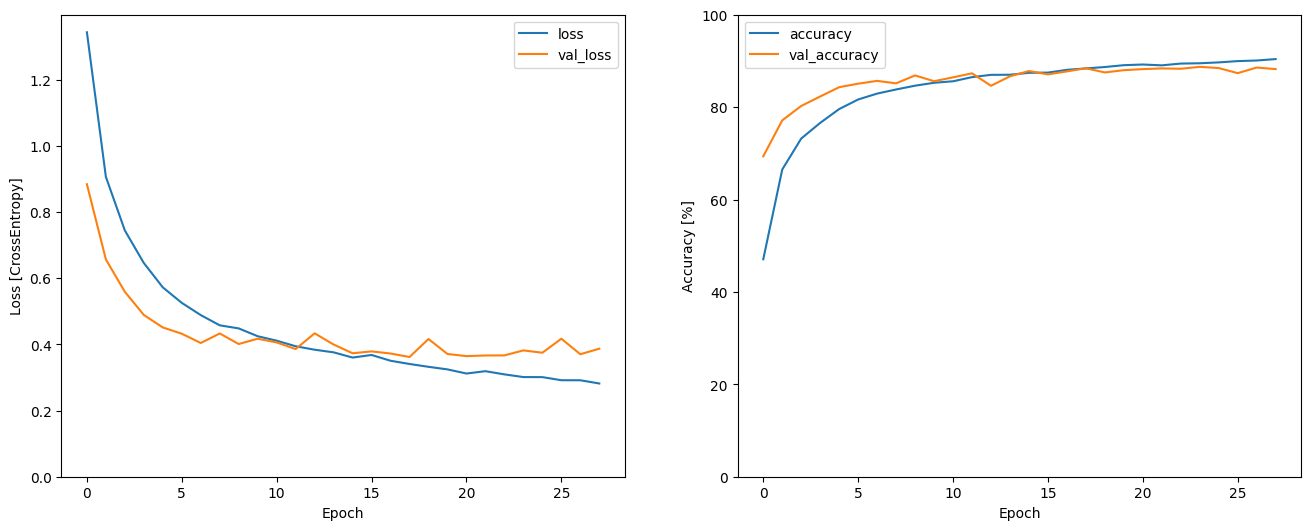
\includegraphics[width=1\linewidth]{Chapters/neuronska_mreza/trening/acc.png} 
    \caption{Gubitak i točnost modela}
    \label{pic:accuracy}
\end{figure}

Konačni iznos funkcije gubitka na testnom skupu iznosi 0.2817, a točnost modela 0.9040, dok
na validacijskom skupu iznosi redom 0.3869 i 0.8823. Međutim, konačna ocjena rezultata
treniranja modela donosi se na temelju testnog skupa. To su podaci koje model nije vidio
niti u jednom trenutku treniranja i predstavljaju podatke kakve će model vidjeti u stvarnom
svijetu. Funkcija gubitka na tom skupu iznosi 0.3480, dok točnost iznosi 0.8814.

Na slici \ref{pic:confmtrx} prikazana je konfuzijska matrica napravljena nad podskupom
testnog skupa podataka. Ona prikazuje koliko je puta model pogriješio u klasifikaciji
određene klase. Stupci matrice predstavljaju stvarne klase, a reci predviđene klase
(izlaz treniranog modela). Na dijagonali matrice nalaze se točne klasifikacije, dok
se izvan dijagonale se nalaze pogreške. Vidljivo je kako je model najviše griješio
u klasifikaciji klase "unknown". To je slučaj zbog toga što se u toj klasi nalaze
zvučni zapisi različitih riječi. Drugim riječima, ta klasa je najraznolikija i najteža
za klasificirati te je zbog toga ovakav rezultat očekivan.

\begin{figure}[htb]
    \centering
    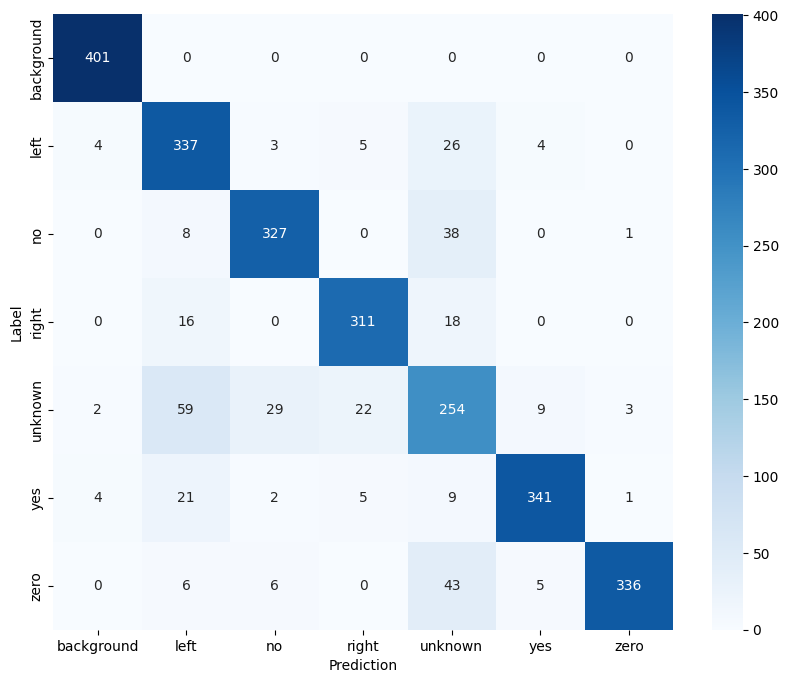
\includegraphics[width=0.7\linewidth]{Chapters/neuronska_mreza/trening/image.png} 
    \caption{Konfuzijska matrica}
    \label{pic:confmtrx}
\end{figure}

\section{Usporedba s drugim modelima na istom skupu podataka}

Usporediti naučeni model s postojećim modelima nije jednostavno zato što
se većina modela temelji na složenijim arhitekturama koje imaju veći broj parametara te
uz svoje rezultate ne prilažu način implementacije na mikrokontroleru. Međutim,
u tablici \ref{tab:models} prikazana je usporedba ovog modela s drugima. Uz naš trenirani model,
ubačen je identičan model treniran na samo dvije glasovne naredbe (ukupno četiri klase).
Iz tablice je vidljivo da naš model zauzima najmanje memorije uz sličnu točnost za 4 klase te
nešto manju za 7 klasa. Točnost bi se jednostavno mogla povećati složenijim potpuno povezanim
slojevima na izlazu trenirane mreže, međutim ovo se čini kao najbolji kompromis između veličine
mreže i njene točnosti.

\begin{table}[htb]
    \centering
    \begin{tabular}{|l|r|r|}
        \hline
        \textbf{Model} & \textbf{Accuracy (\%)} & \textbf{Model Size (KB)} \\ \hline
        Naš CNN (7 klasa) & 88.2 & 15.7 \\ 
        Naš CNN (4 klase) & 93.6 & 15.6 \\ 
        DNN (Deep Neural Network)          \cite{zhang2017hello} & 84.6 & 80 \\
        CNN (Convolutional Neural Network) \cite{zhang2017hello} & 91.6 & 79 \\
        LSTM (Long Short-Term Memory)      \cite{zhang2017hello} & 92.9 & 79.5 \\
        CRNN (Convolutional RNN)           \cite{zhang2017hello} & 94.0 & 79.7 \\
        DS-CNN (Depthwise Separable CNN)   \cite{zhang2017hello} & 94.4 & 38.6  \\
        TripletLoss-res15 \cite{triplet} & 95.2 & 237 \\
        BC-ResNet-8 \cite{res} & 98.7 & 520 \\
        WaveFormer \cite{waveformer} & 98.8 & 130  \\
        \hline
    \end{tabular}
    \caption{Veličine različitih oblika modela i procentualna ušteda}
    \label{tab:models}
\end{table}
